% Verbatim draft import from camera-ready.tex.
% Section levels and labels are adjusted for thesis inclusion under Section 3.5.

In this section, we shifted our focus towards logical reasoning: deductively inferring the truth value of a
conclusion from a collection of premises. Prior to our work, there had been many prompting and chain-of-thought based
strategies to improve the logical reasoning capabilities of language models. However, we found that they
failed in subtle and unpredictable ways. To mitigate this, we introduced \texttt{LINC}: \textbf{L}ogical
\textbf{I}nference via \textbf{N}eurosymbolic \textbf{C}omputation.

In \texttt{LINC}, logical reasoning is tackled through a two-step neurosymbolic process.
In the first step, a language model takes the natural language premises and desired conclusion and converts them into first-order logic (FOL) expressions \cite{enderton2001mathematical, barker-plummer2011language}.
Once everything is represented in first-order logic, we then apply a symbolic theorem prover to determine the truth value of the conclusion.
As the translation from natural language to first-order logic can be imperfect, we use a majority voting scheme to
improve the reliability of the approach.

The key advantage of \texttt{LINC} is that the reasoning burden is offloaded from the language model to the theorem prover.
On the other hand, the challenge shifts to faithful and accurate formalization. The FOL translation must capture all the relevant
information from the premises without adding or removing any information. Since it is not clear how the difficulties of formalization
and natural language reasoning compare, the main focus of our work was to compare and contrast \texttt{LINC} with traditional
\texttt{Chain-of-Thought} approaches. Through thorough experimentation and analysis on two challenging datasets,
we provided insights into the strengths and weaknesses of both approaches. Overall, we found that they have distinct behaviors and
failure modes, suggesting a strong synergy between theorem provers and language models.


\begin{figure}[ht!]
  \centering
  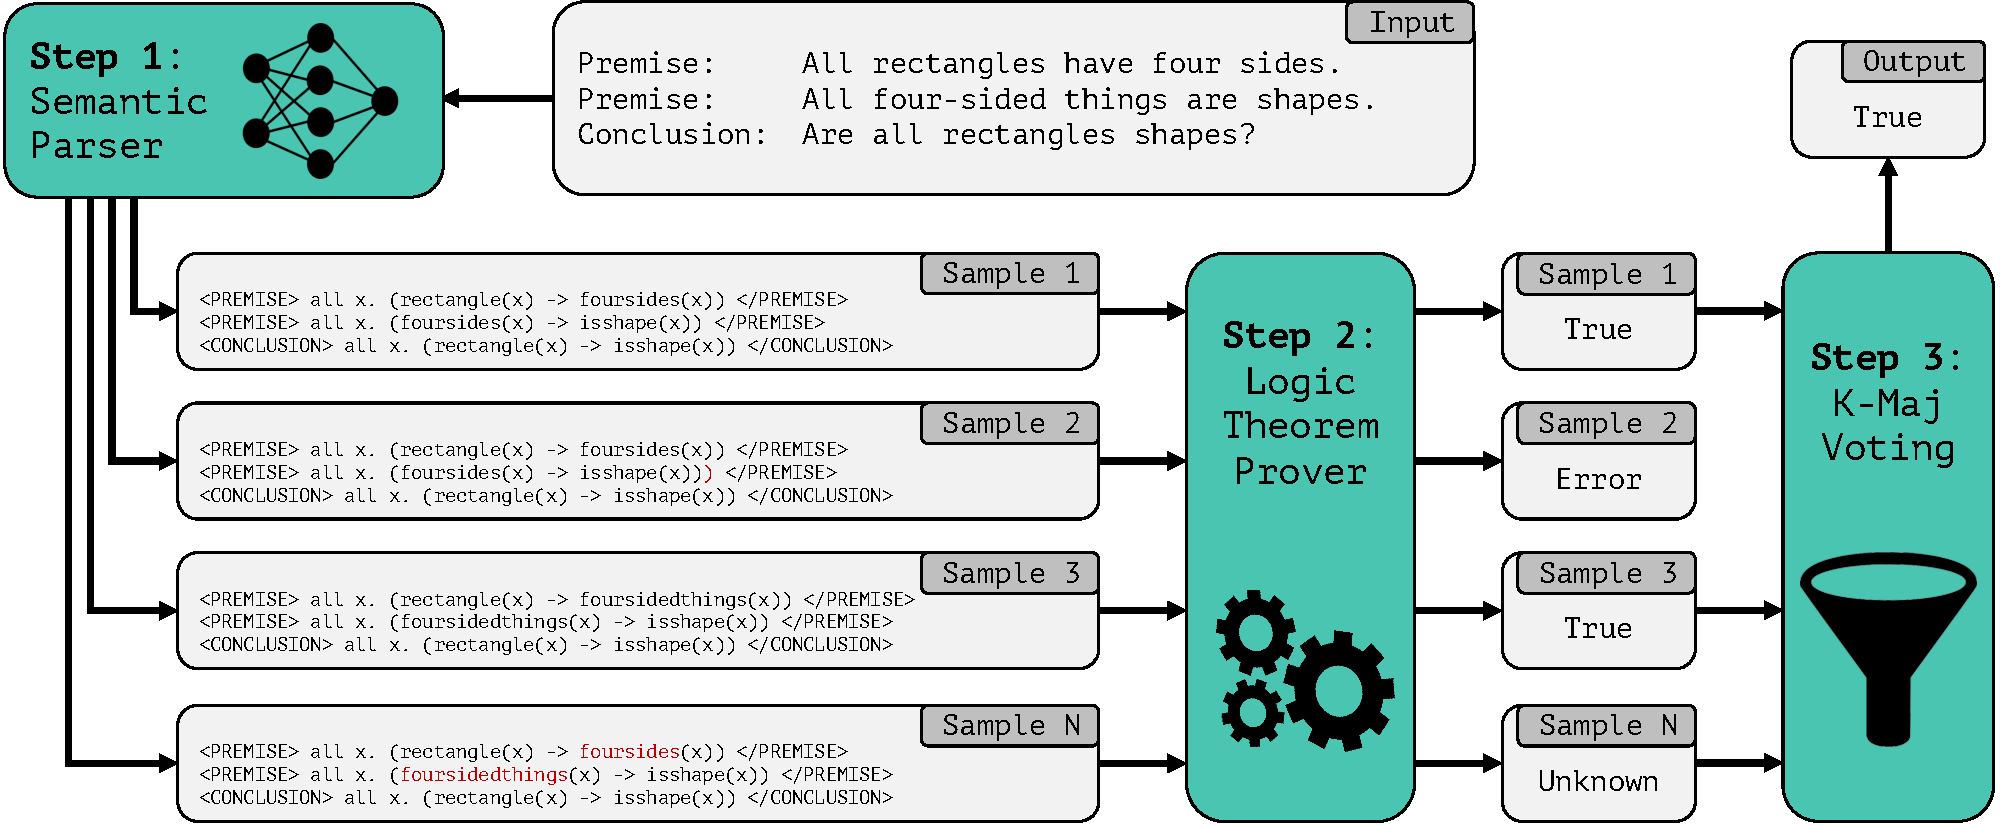
\includegraphics[width=\linewidth]{figures/pipeline.pdf}
  \caption{Overview of the \texttt{LINC} approach. Starting from a problem in natural language, the language model first samples first-order logic translations of the premises and conclusion. The translated formulas are then passed to an automated theorem prover, which filters invalid syntax and predicts labels for the valid samples. Finally, a majority-vote step aggregates the remaining candidate labels.}
  \label{linc-paper:fig:main}
\end{figure}

%%%
\subsection{\texttt{LINC}: Logical Inference via Neurosymbolic Computation}
\label{linc-paper:sec:ns-model}

Fig.~\ref{linc-paper:fig:main} provides an overview of \texttt{LINC}'s two-stage approach.
First, the LLM acts as a semantic parser to generate first-order logic expressions to be sent to the automated theorem prover.
Second, \texttt{Prover9} \citep{prover9-mace4} executes the expressions to determine whether the conclusion is \texttt{True},
\texttt{False}, or \texttt{Uncertain} under the translated premises, and raises an exception if the FOL syntax is
invalid. The $K$-Maj voting scheme then aggregates predictions across multiple samples to determine the final prediction.

The core tradeoff of \texttt{LINC} is that the difficulty is shifted from faithful reasoning to faithful formalization.
Using \texttt{LINC}, a language model no longer needs to reason in natural language. This
removes any reasoning errors that may arise from the model's inability to properly keep
of logical structure. On the other hand, with \texttt{LINC}, the model must now faithfully formalize
each of the natural language statements into FOL. This requires the FOL expressions to both be 1) \textit{syntactically}
valid, so that they are accepted by the prover, and 2) \textit{semantically} valid, so that they contain the same semantic information
as the natural language statements. As shown later in the error analysis, this translation can be difficult when statements are more complex,
because the FOL expressions may fail to capture both explicit and implicit information.

%%%
\subsection{Experiments}\label{linc-paper:sec:experiments}
In this section, we present our experimental setup, the models we used, and the three baselines to which we compared \texttt{LINC}.

\textbf{Datasets:} We used two challenging datasets for logical reasoning in natural language: \textbf{FOLIO} \cite{han2022folio} and \textbf{ProofWriter} \cite{tafjord2021proofwriter}.
FOLIO is an expert-written, open-domain, logically complex and diverse dataset for natural
language reasoning with first-order logic. We used the validation set but discovered that 22 of the 204 samples contain errors
(details in the original paper appendix), so we used the other 182 samples.
ProofWriter is a synthetically generated dataset for logical reasoning over natural language.
We randomly selected 360 samples from the OWA (Open-World Assumption) subset of ProofWriter in
a way that is balanced across the number of reasoning steps in the shortest ground truth proof
(depth 0-5; 50 samples each) and across the three labels (120 samples each; 20 each per depth).

\textbf{In-context learning examples:} We hand-picked eight diverse samples from the FOLIO training set
to be used as few-shot in-context examples. Because ProofWriter does not come with ground truth
FOL statements, we used these eight samples for both evaluations. Questions in
ProofWriter generally have more premises per question than in FOLIO (5.3 in FOLIO vs. 18.8 in ProofWriter).
Thus, our evaluation on FOLIO is an \emph{in-distribution} task, whereas ProofWriter
requires generalizing \emph{out-of-distribution} to reasoning over considerably larger
sets of premises than are given in the prompt.

\textbf{Majority voting:} We used $K$-way majority voting \cite{wang2023self}, where $K$ samples are taken i.i.d. from the model and the mode used as the final prediction.
We reported $K{=}10$-way majority voting unless otherwise stated, with ties broken arbitrarily.
We reported the effect of $K$ on performance across our conditions and briefly discussed trends in the original paper appendix.

\textbf{Models:}
We used three models pre-trained on both natural language and code: GPT-3.5 \citep{ouyang2022training}, GPT-4 (\texttt{gpt-3.5-turbo-16k-0613} and \texttt{gpt-4-0613}) \citep{openai2023gpt4}, and StarCoder+ (\url{https://huggingface.co/bigcode/starcoderplus}) \citep{li2023starcoder} with a decoding temperature of $T=0.8$ for all experiments. We defer model, hyperparameter, and hardware details to the original paper appendix.
We opted for \texttt{StarCoder+} for three reasons: firstly, unlike the other models we considered, it is a free, open-access model. Secondly, it has a dataset search functionality (see \url{https://huggingface.co/spaces/bigcode/in-the-stack} and \url{https://huggingface.co/spaces/bigcode/search}), with which we verified that FOLIO and ProofWriter were not in \texttt{StarCoder+}'s training set, giving further assurance in the validity of our findings. Thirdly, with its 15.5B parameters it is likely considerably smaller than GPT-3.5 and GPT-4; although the exact size of these models has not been made public, their common predecessor GPT-3 was known to have 175B parameters \citep{brown2020language}. This allowed us to compare performance at different model scales.

\textbf{Controlled baselines:}

\begin{figure}[ht!]
  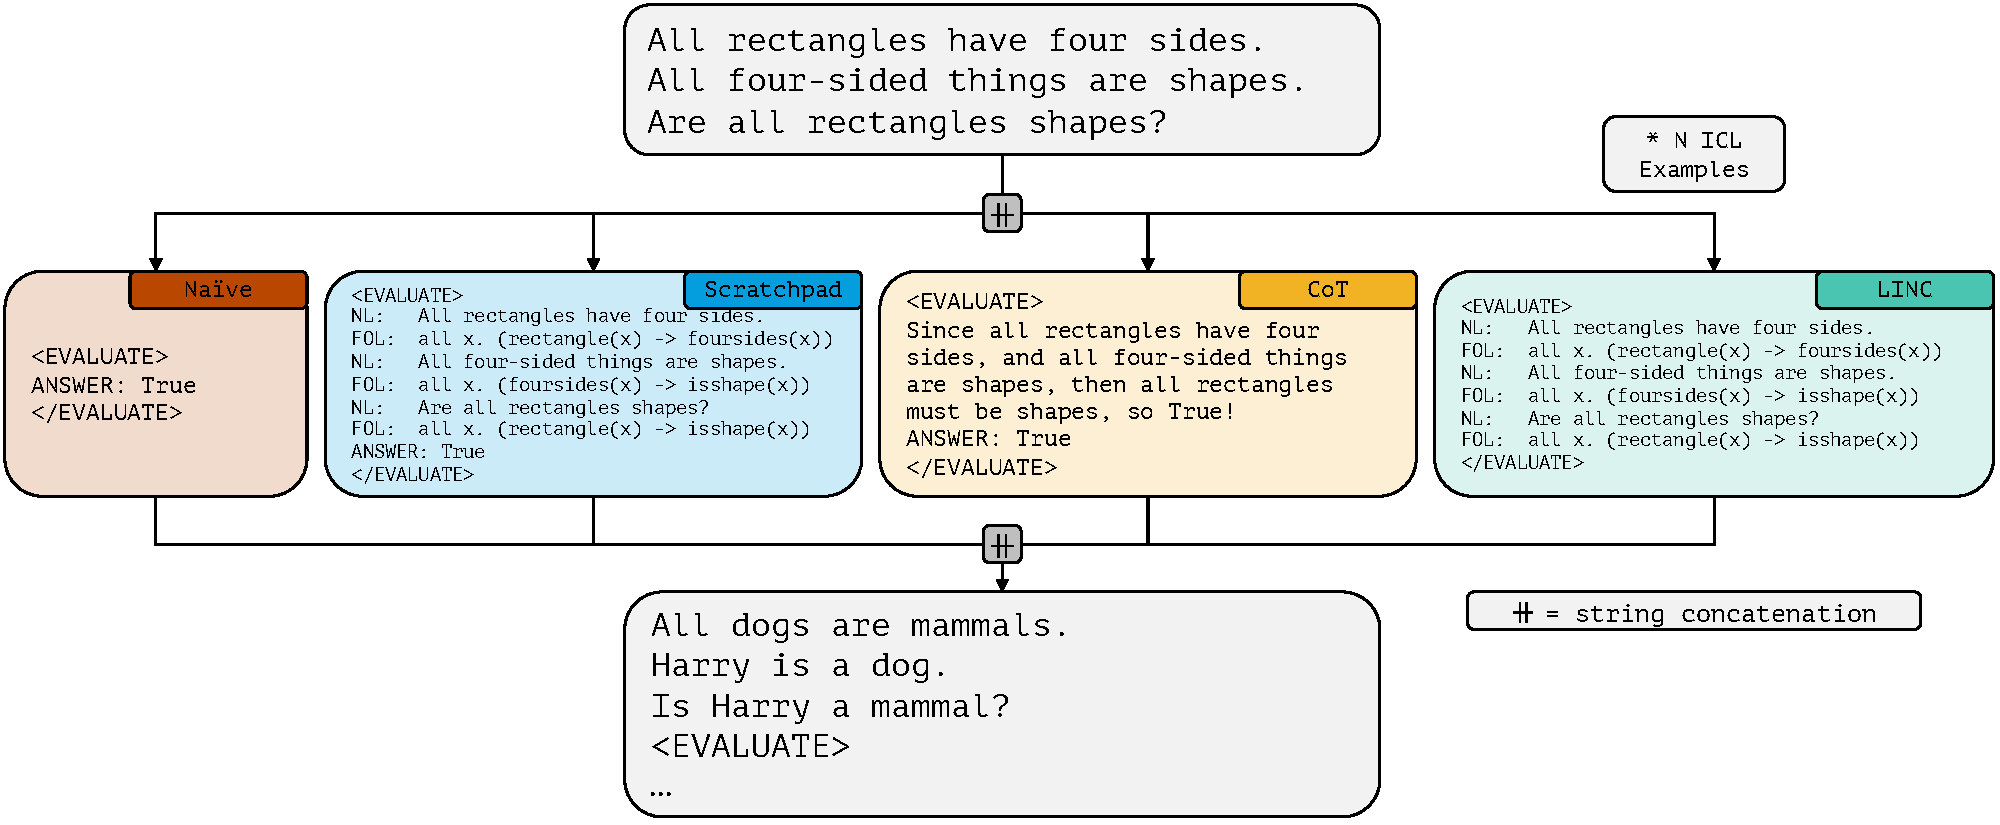
\includegraphics[width=\linewidth]{figures/prompt.pdf}
  \caption{This figure outlines the string concatenation workflow for each of our conditions. We start with the original problem, provide ICL examples through an intermediate markup language, and finally append the problem to evaluate. At this stage, we allow the model to autoregressively sample until producing a stop token.}
  \label{linc-paper:fig:prompt}
\end{figure}
\label{linc-paper:sec:controlled-baselines}
As shown in Fig.~\ref{linc-paper:fig:prompt}, we compared LINC with three baseline approaches: \texttt{Na\"ive}, \texttt{Scratchpad}, and \texttt{Chain-of-Thought (CoT)}.
In \texttt{Na\"ive} (red), the model is given the natural language premises and asked to directly generate the label (\texttt{True}/\texttt{False}/\texttt{Uncertain}).
In \texttt{Scratchpad} (blue) \cite{nye2021show}, we ablated the effectiveness of using a symbolic prover instead of a LLM in the second stage.
The model is asked to generate FOL expressions just like in LINC, but instead of passing the FOL expressions to a symbolic prover, we ask the model to directly predict the label based on its own FOL translation.
In \texttt{CoT} (yellow), we used standard \texttt{CoT} prompting \cite{wei2022chain,kojima2022large,wang2023self}, where the model is asked to generate step-by-step natural language reasoning to arrive at the conclusion.
The prompts we used for all approaches can be found in the original paper appendix.

\begin{figure}[th]
  \centering
  \begin{subfigure}[b]{0.45\textwidth}
    \centering
    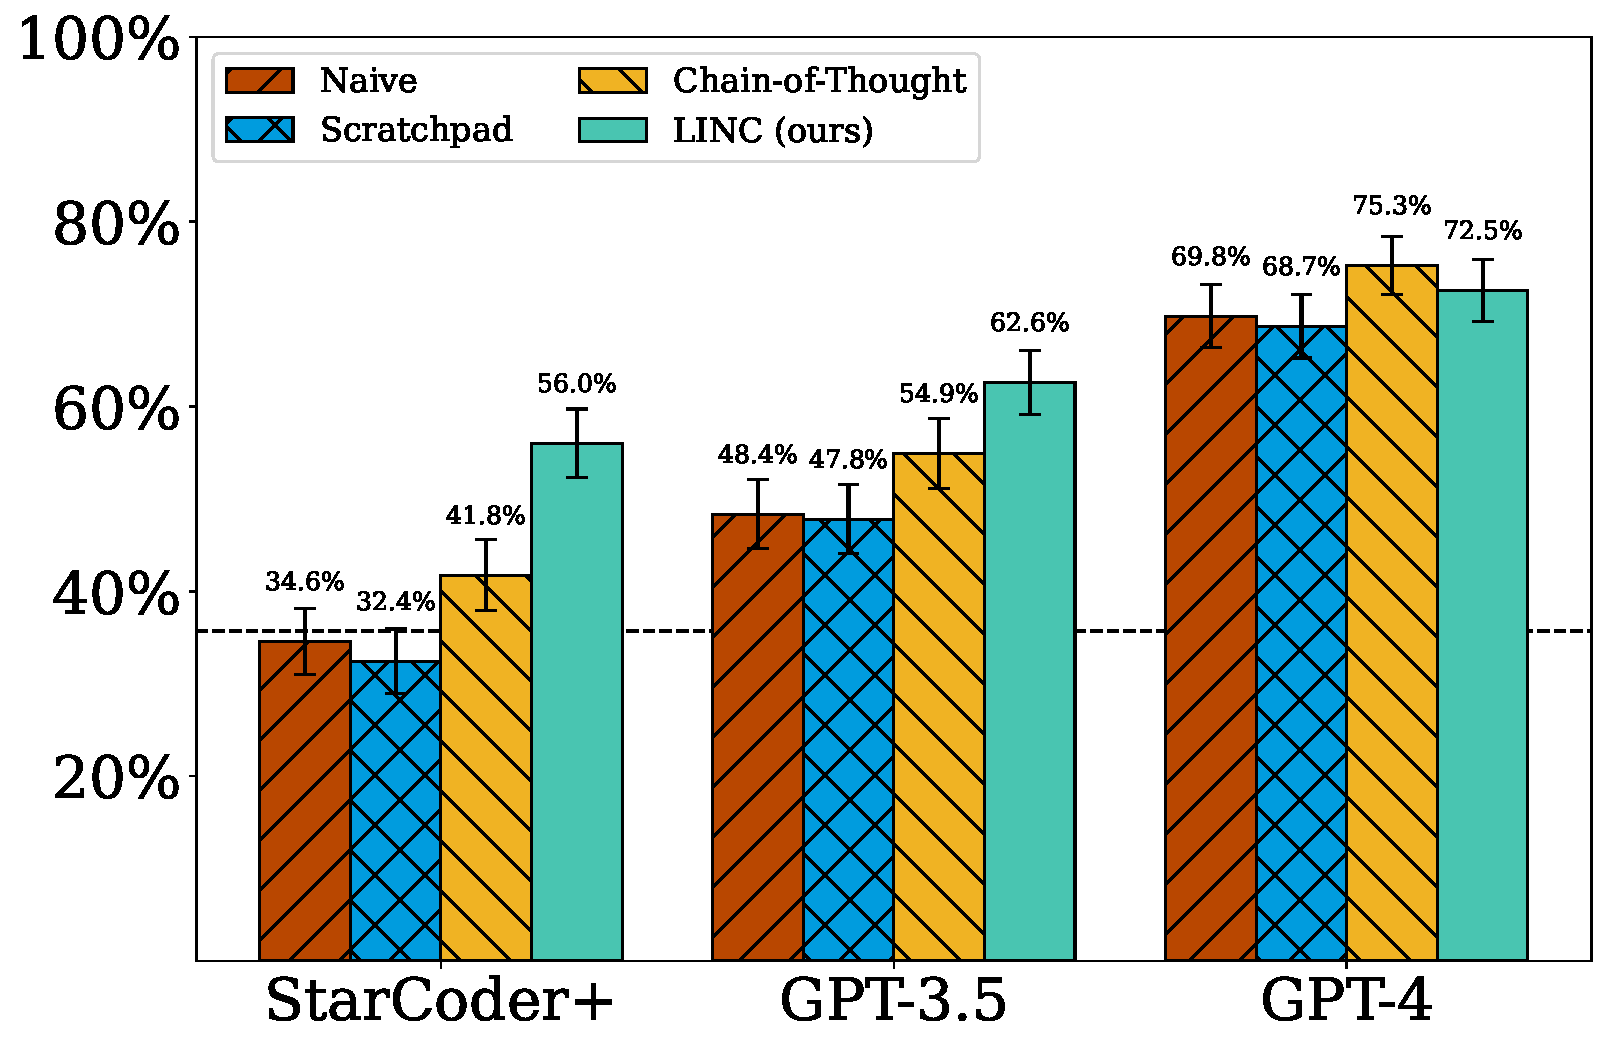
\includegraphics[width=\textwidth]{figures/folio_bar_chart.pdf}
    \caption{FOLIO.}
    \label{linc-paper:fig:results-folio}
  \end{subfigure}
  \hfill
  \begin{subfigure}[b]{0.45\textwidth}
    \centering
    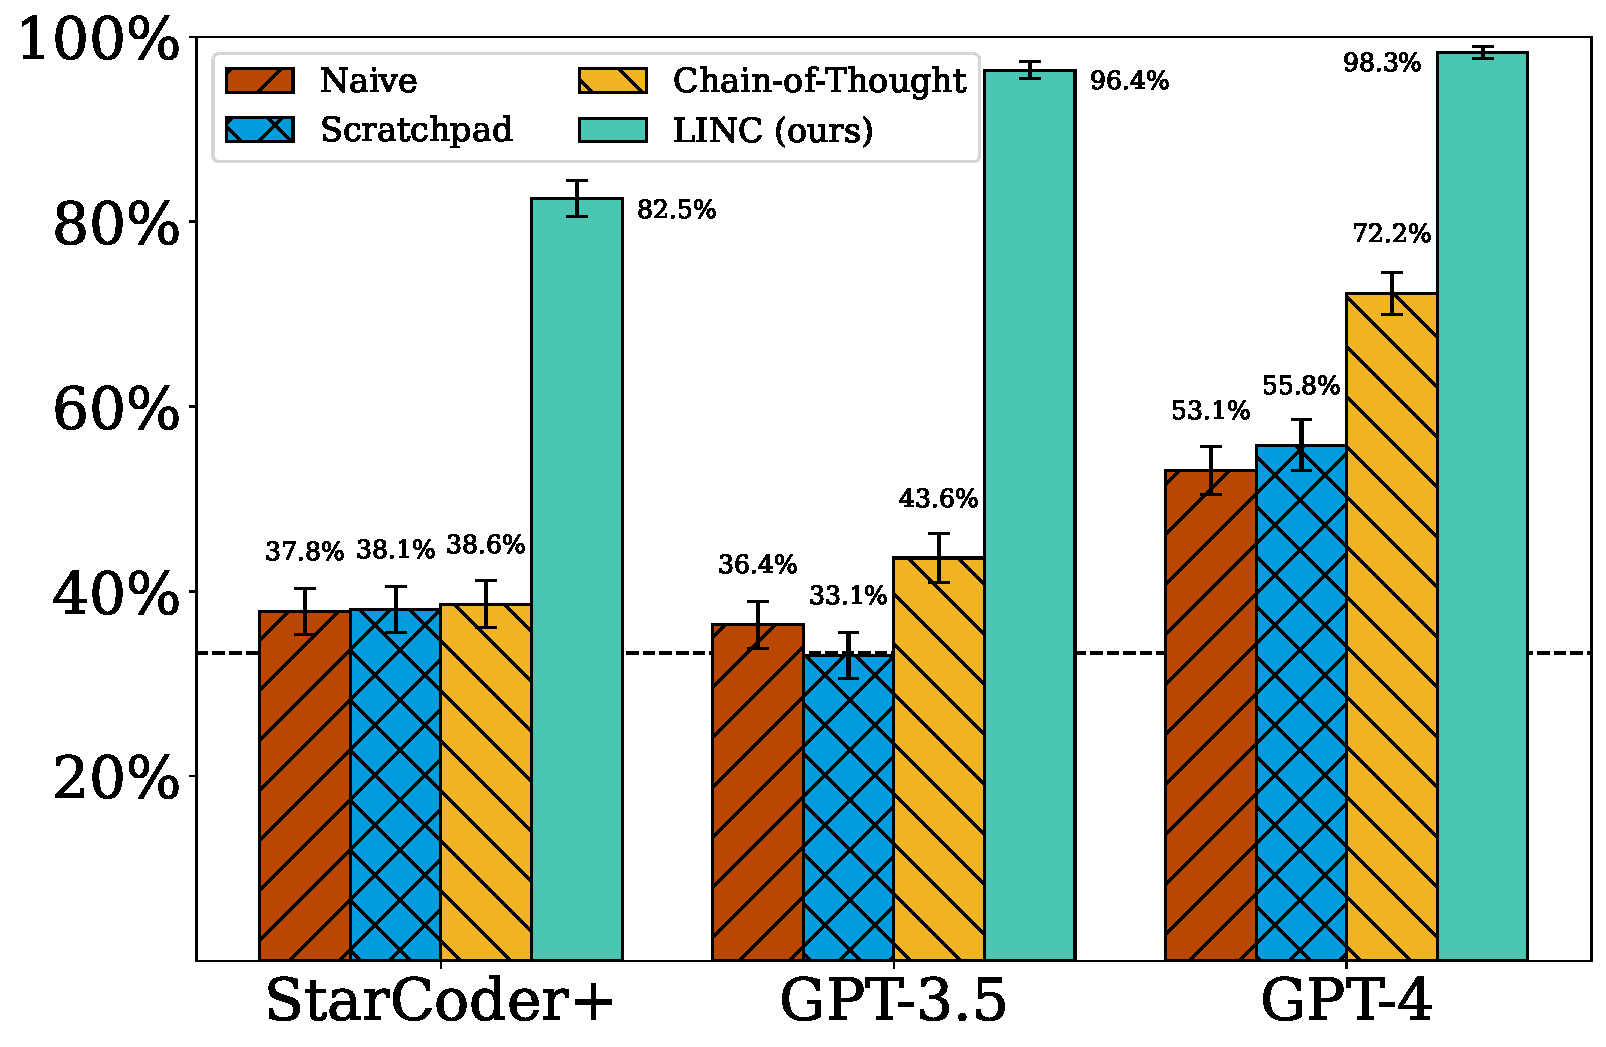
\includegraphics[width=\textwidth]{figures/proofwriter_bar_chart.pdf}
    \caption{ProofWriter.}
    \label{linc-paper:fig:results-pw}
  \end{subfigure}
  \caption{Results of each model on the FOLIO and ProofWriter datasets. Accuracies are for bootstrapped $10$-way majority vote for all models. Error bars are $\pm 1$ bootstrapped standard deviation. Dotted, black line is the accuracy obtained by always guessing the most common label in the dataset.}
  \label{linc-paper:fig:results-main}
\end{figure}

%%%
\subsection{Results \& Discussion}
\label{linc-paper:sec:results_discussion}

Our main results are shown in Figure~\ref{linc-paper:fig:results-main}.
Each bar represents either \texttt{LINC} or one of the three baselines,
while each group of bars indicates the language model used (in \{\texttt{StarCoder+}, \texttt{GPT-3.5}, \texttt{GPT-4}\}).

On FOLIO (Figure \ref{linc-paper:fig:results-folio}), StarCoder+---the smallest model we experimented with---benefited the most from \texttt{LINC}, achieving a mean accuracy that was 14.2 points higher than the closest controlled baseline (56.0\% vs. 41.8\% with \texttt{CoT}).
We found that \texttt{Scratchpad}, where the intermediate logical formulae are still generated but the call to the symbolic solver is ablated and replaced by the model's own prediction, did not appear to benefit performance; for StarCoder+, neither \texttt{Scratchpad} nor the \texttt{Na\"ive} baseline performed better than simply deterministically predicting the most common label (``\texttt{Uncertain}'').
For GPT-3.5, the trend is similar, although the gap between \texttt{LINC} and the closest baseline shrinks (62.6\% vs. 54.9\% average accuracies).
For GPT-4, the trend reversed: \texttt{LINC} underperformed \texttt{CoT}. However, we performed a McNemar's test \cite{mcnemar1947note} to get the p-value on this GPT-4 \texttt{LINC} vs. \texttt{CoT} comparison, and we found that the difference was not significant ($p=0.58$).
Meanwhile, for our balanced subset of ProofWriter, we saw significant performance gains across the board (Figure \ref{linc-paper:fig:results-pw}); particularly so for GPT-3.5 and GPT-4, which achieved mean accuracies of 96.4\% and 98.3\% when paired with LINC.

We attribute the superior performance of \texttt{LINC} on ProofWriter to two causes.
First, ProofWriter is much easier to formalize than FOLIO, which is the bottleneck for LINC.
While FOLIO contains complex sentences with linguistic variety, all sentences in ProofWriter are synthetically generated and easily formalizable.
Second, ProofWriter is an \emph{out-of-distribution} setting, where the in-context examples contain fewer premises and shorter deductive chains than the
reasoning task.
This distribution shift makes it harder for the model to ignore irrelevant premises and keep track of the long deductive chains.
By removing the reasoning burden, \texttt{LINC} is able to ignore this difficulty and perform well.

\begin{figure}[th]
  \centering
  \begin{subfigure}[b]{0.32\textwidth}
    \centering
    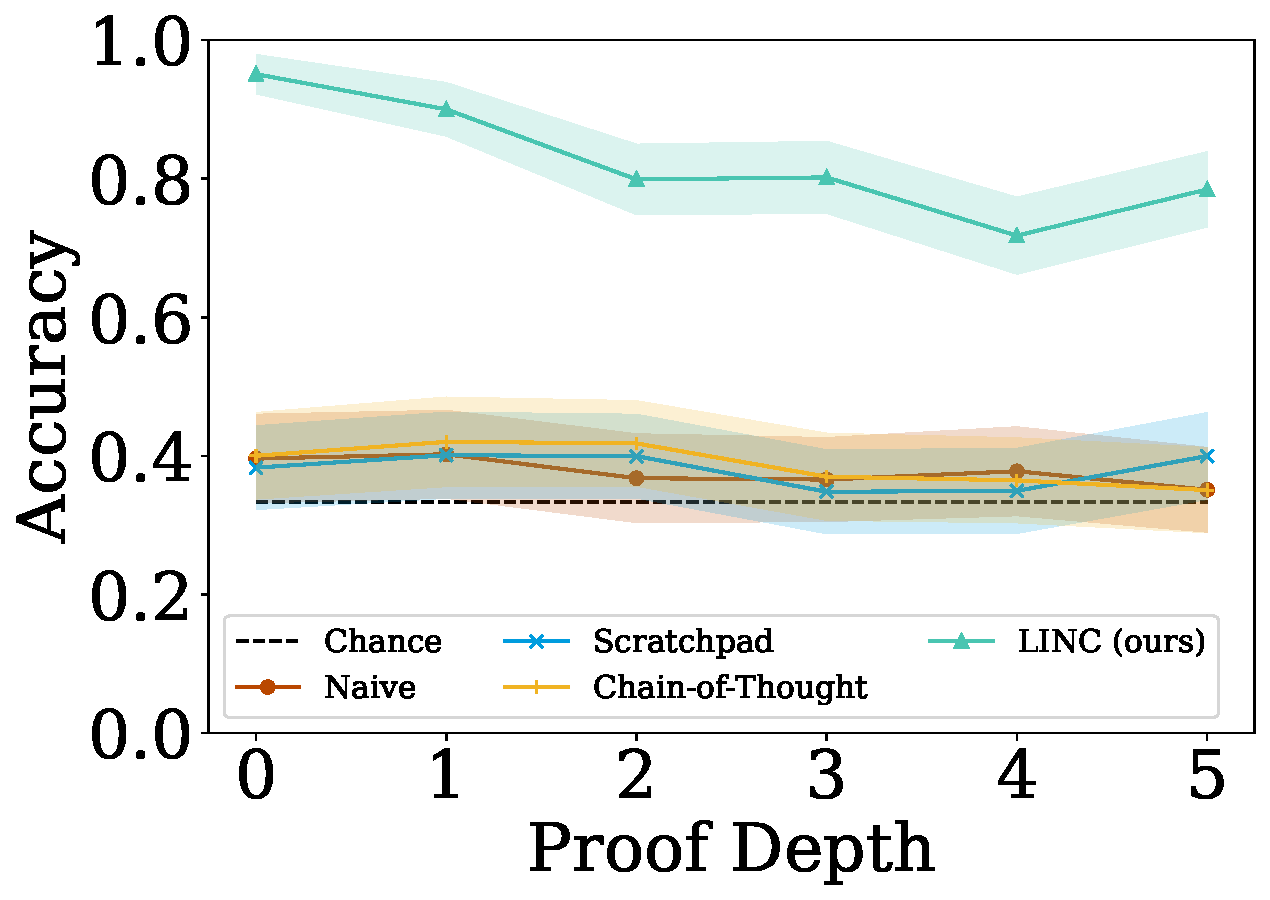
\includegraphics[width=\textwidth]{figures/starcoderplus_qdep_line_plot.pdf}
    \caption{StarCoder+.}
    \label{linc-paper:fig:starcoder-qdep}
  \end{subfigure}
  \hfill
  \begin{subfigure}[b]{0.32\textwidth}
    \centering
    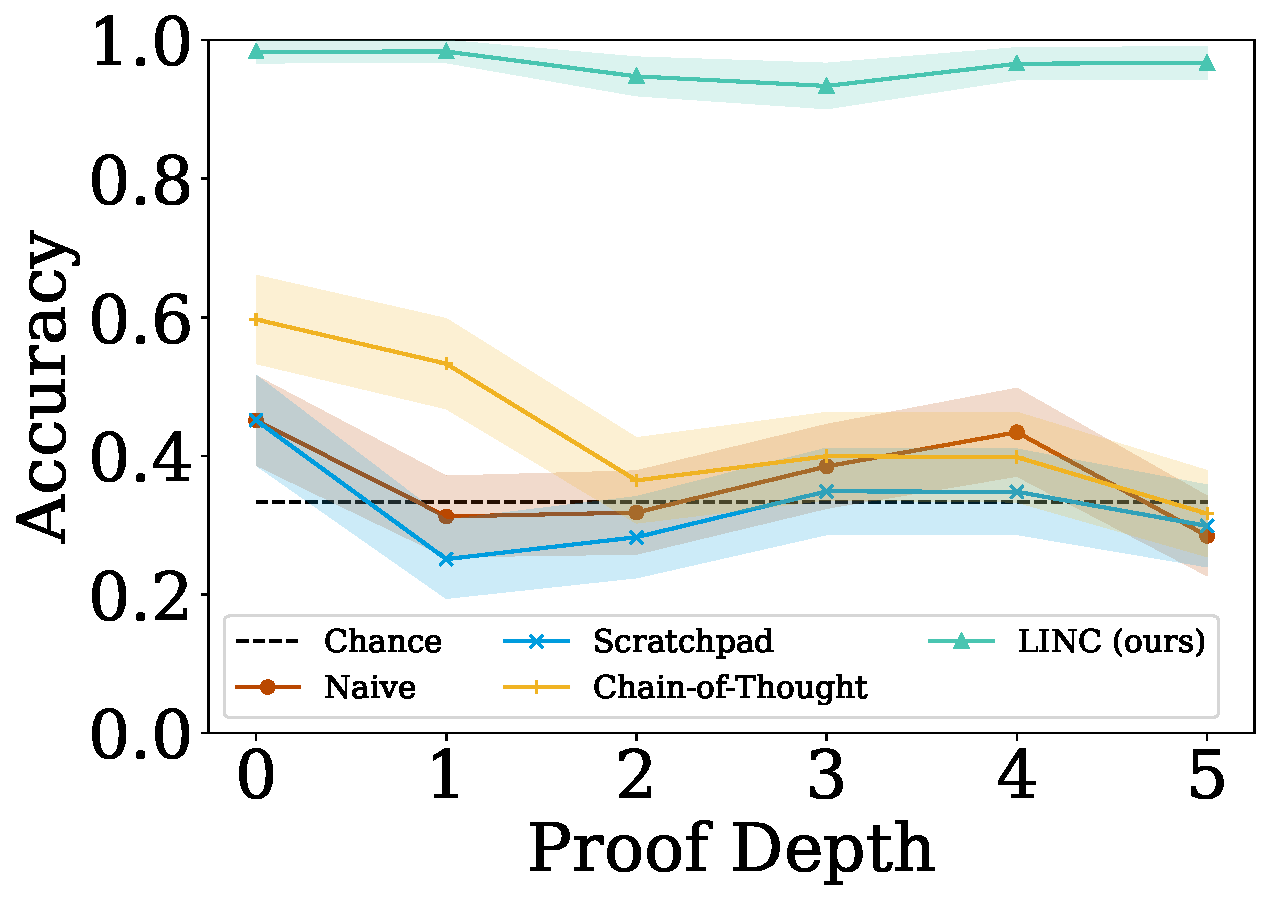
\includegraphics[width=\textwidth]{figures/gpt-3.5-turbo-16k-0613_qdep_line_plot.pdf}
    \caption{GPT-3.5.}
    \label{linc-paper:fig:gpt-3.5-qdep}
  \end{subfigure}
  \hfill
  \begin{subfigure}[b]{0.32\textwidth}
    \centering
    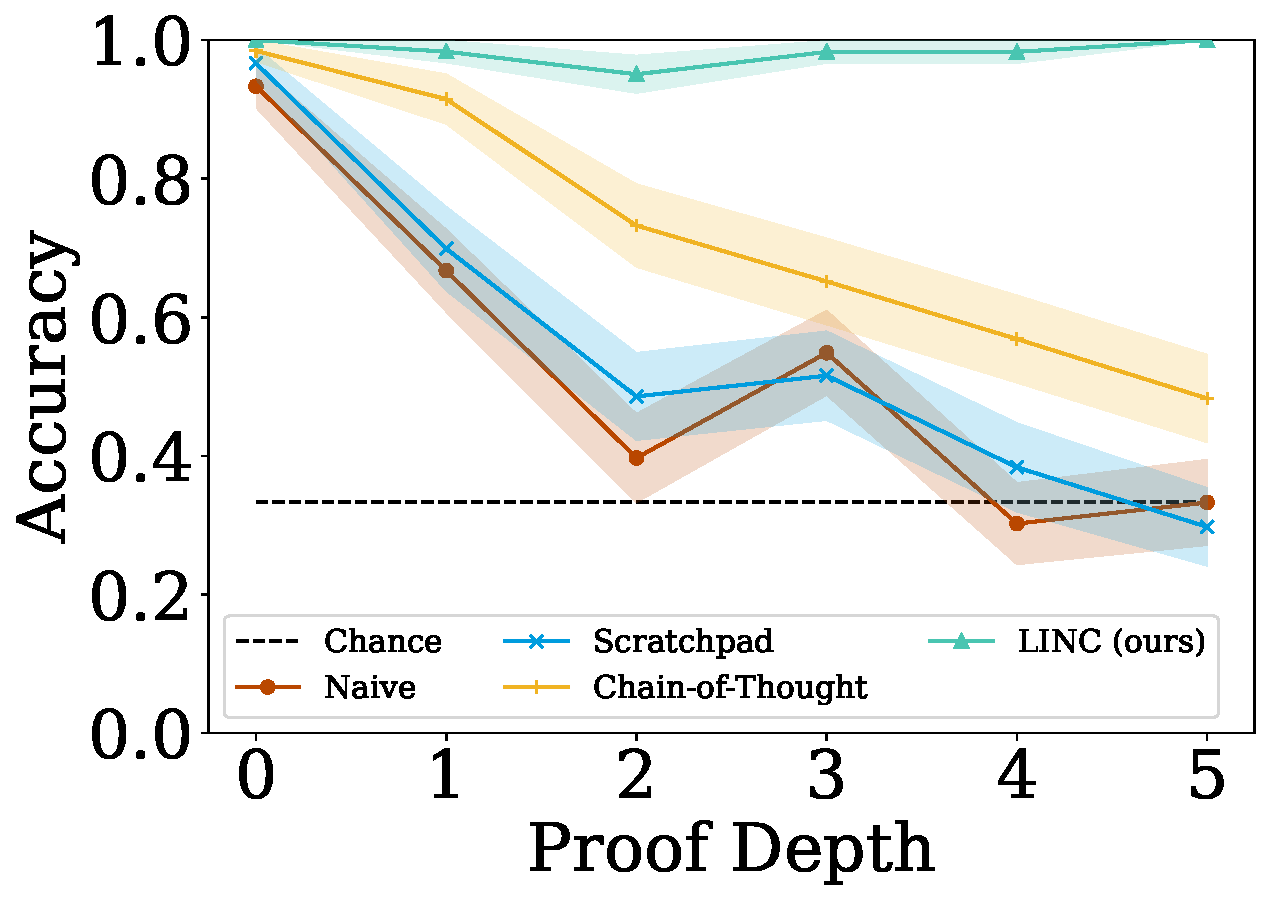
\includegraphics[width=\textwidth]{figures/gpt-4-0613_qdep_line_plot.pdf}
    \caption{GPT-4.}
    \label{linc-paper:fig:gpt-4-qdep}
  \end{subfigure}
  \caption{Accuracy per necessary proof depth in ProofWriter. Accuracies reported are for bootstrapped $10$-way majority vote, and shaded areas cover $\pm 1$ bootstrapped standard deviation. Black, dotted lines reflect the expected success rate of guessing a random label, which is 1/3 in all subsets per our experiment design.}
  \label{linc-paper:fig:results-qdep}
\end{figure}

Finally, in Figure~\ref{linc-paper:fig:results-qdep} we analyzed each model's performance on ProofWriter as a function of the necessary proof depth.
First, we found that StarCoder+'s performance was close to random chance across all three baselines, suggesting it did not have reasoning capabilities out-of-the-box.
With \texttt{LINC}, it attains almost perfect accuracy at depths $0$ and $1$, but drops as the necessary proof length increases, likely due to some formalization inaccuracies.
As StarCoder+ is a coding model, it makes sense that its formalization abilities far exceed its reasoning abilities.
For GPT-3.5, all baselines perform above chance at depth $0$, but quickly drop down for higher proof depths. In contrast,
\texttt{LINC} allows it to achieve near-perfect performance for all proof depths, showing our approach scales even for longer reasoning chains.
We saw a similar trend for GPT-4: although the baselines were significantly stronger, reasoning difficulty still remained at larger proof depths.

\begin{figure}[th]
  \centering
  \begin{subfigure}[b]{0.48\textwidth}
    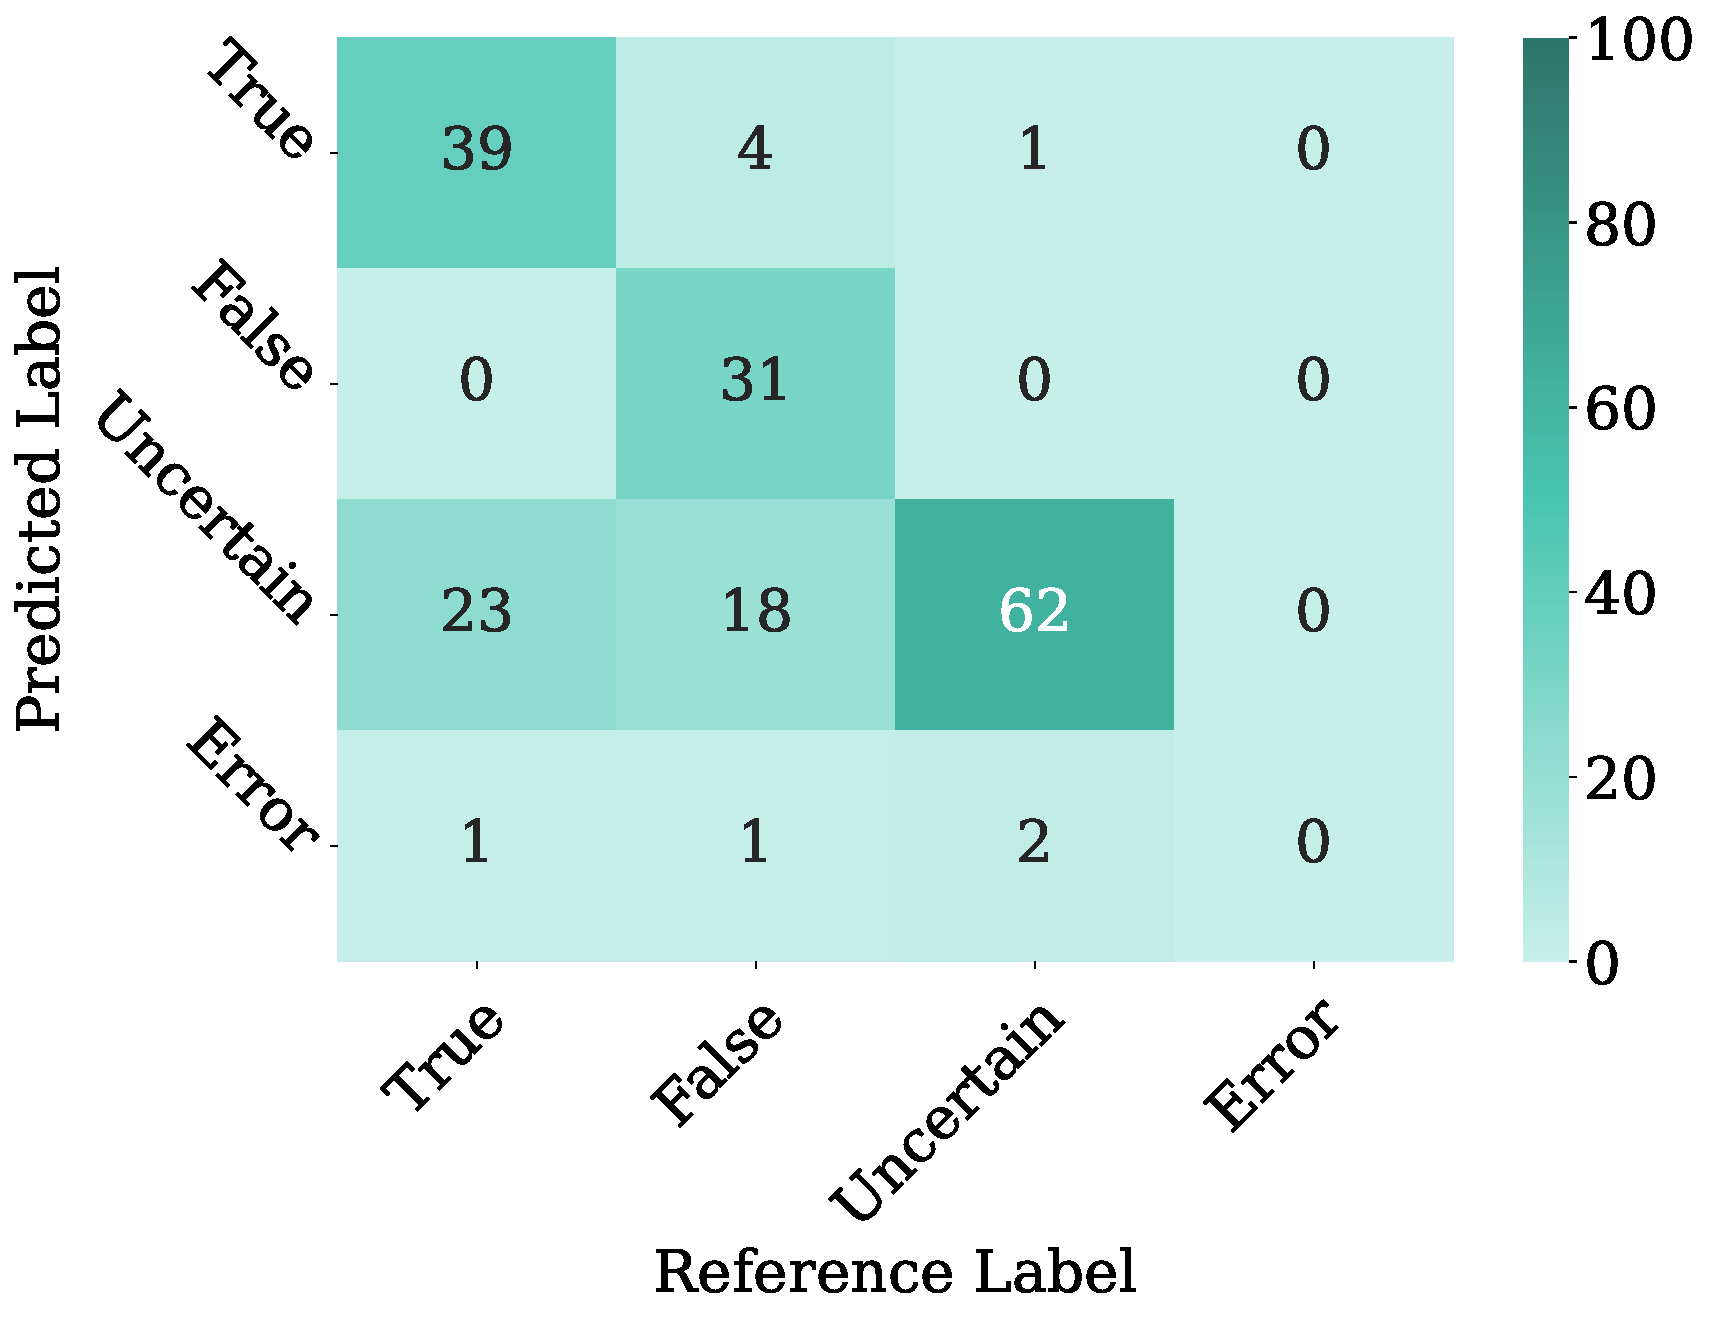
\includegraphics[width=\textwidth]{figures/matrices/gpt4_neurosym_confusion.pdf}
    \caption{Confusion matrix for \texttt{LINC}.}
    \label{linc-paper:fig:gpt_neurosym_confusion}
  \end{subfigure}
  \hfill
  \begin{subfigure}[b]{0.48\textwidth}
    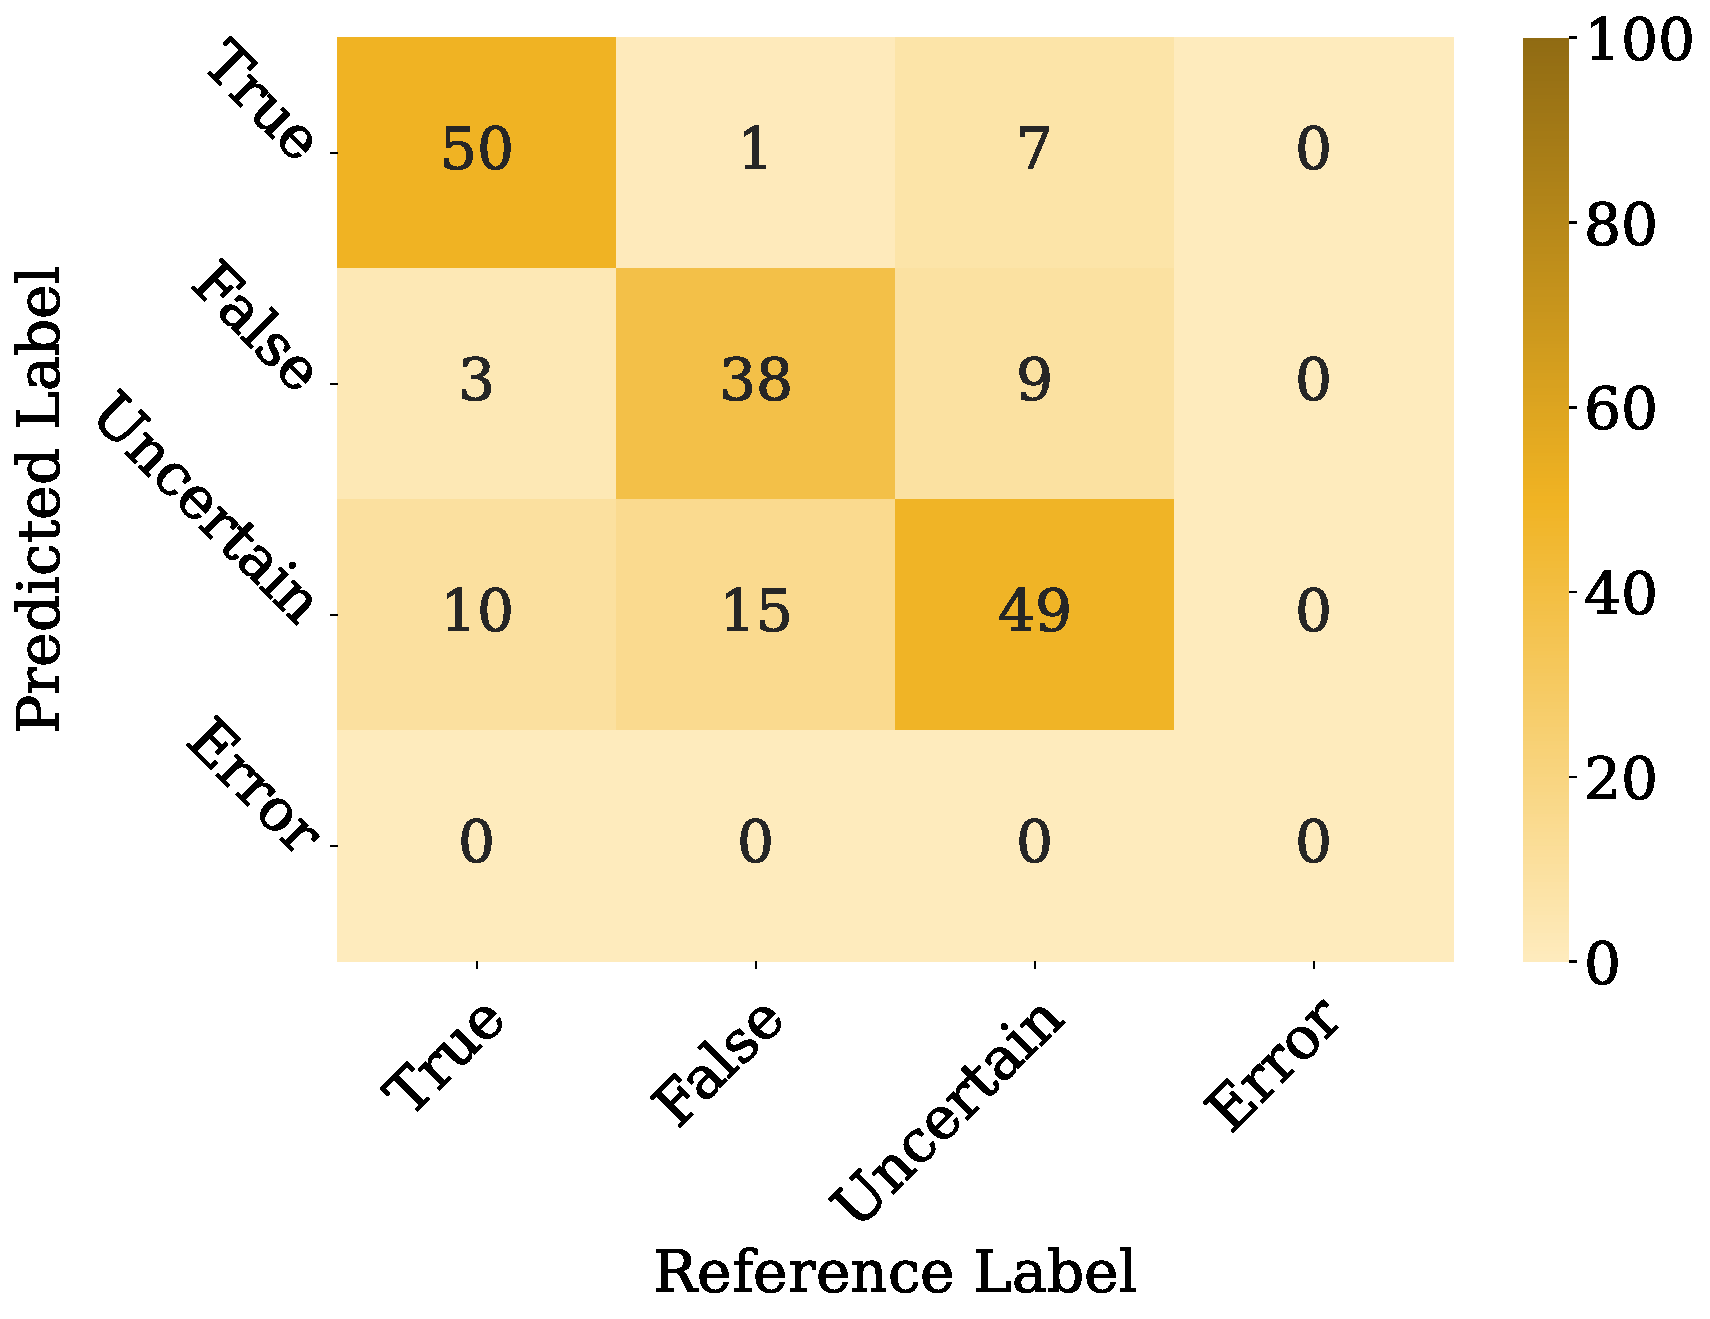
\includegraphics[width=\textwidth]{figures/matrices/gpt4_cot_confusion.pdf}
    \caption{Confusion matrix for \texttt{Chain-of-Thought}.}
    \label{linc-paper:fig:gpt_cot_confusion}
  \end{subfigure}
  \hfill
  \begin{subfigure}[b]{0.48\textwidth}
    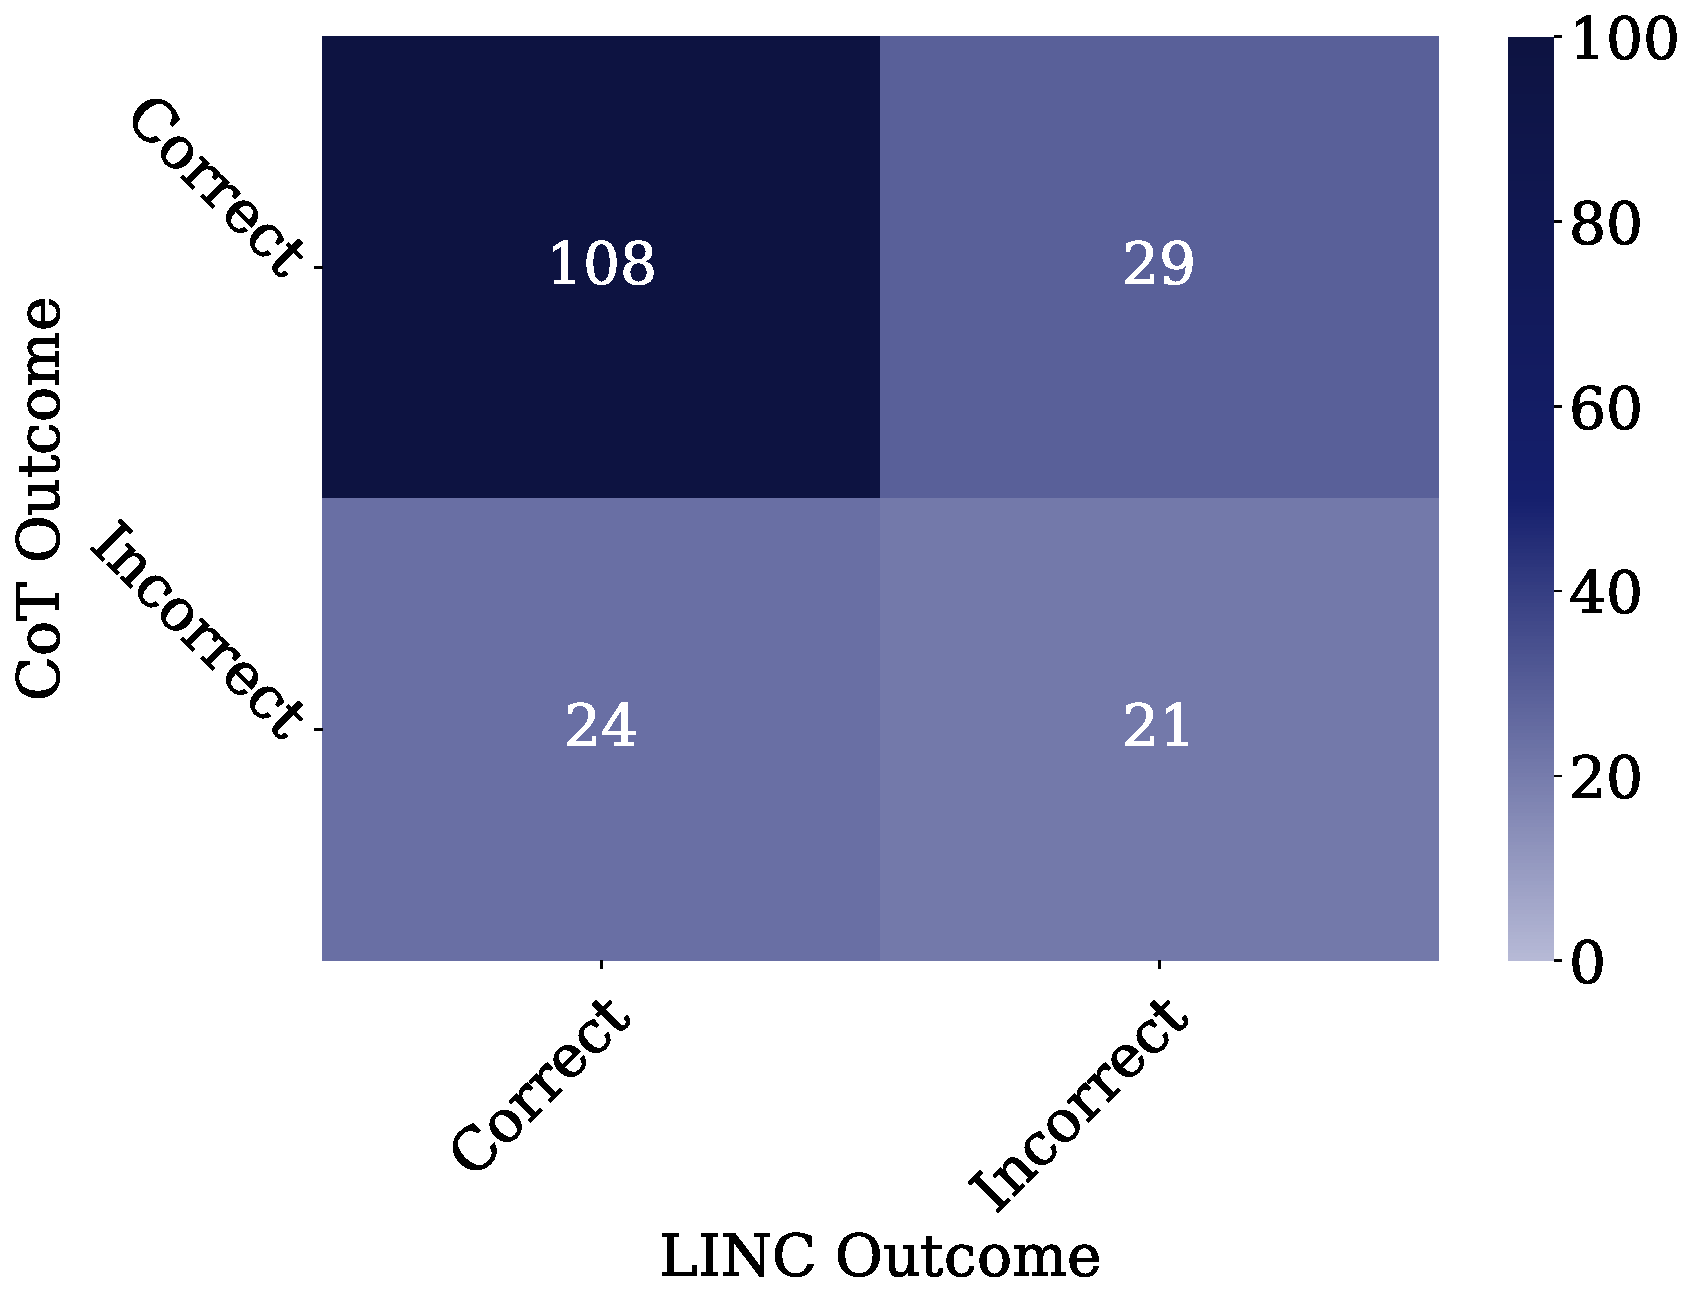
\includegraphics[width=\textwidth]{figures/matrices/gpt-4_cot_neurosym.pdf}
    \caption{Comparing the consistency of \texttt{LINC} vs. \texttt{Chain-of-Thought}.}
    \label{linc-paper:fig:gpt_cot_neurosym}
  \end{subfigure}
  \hfill
  \begin{subfigure}[b]{0.48\textwidth}
    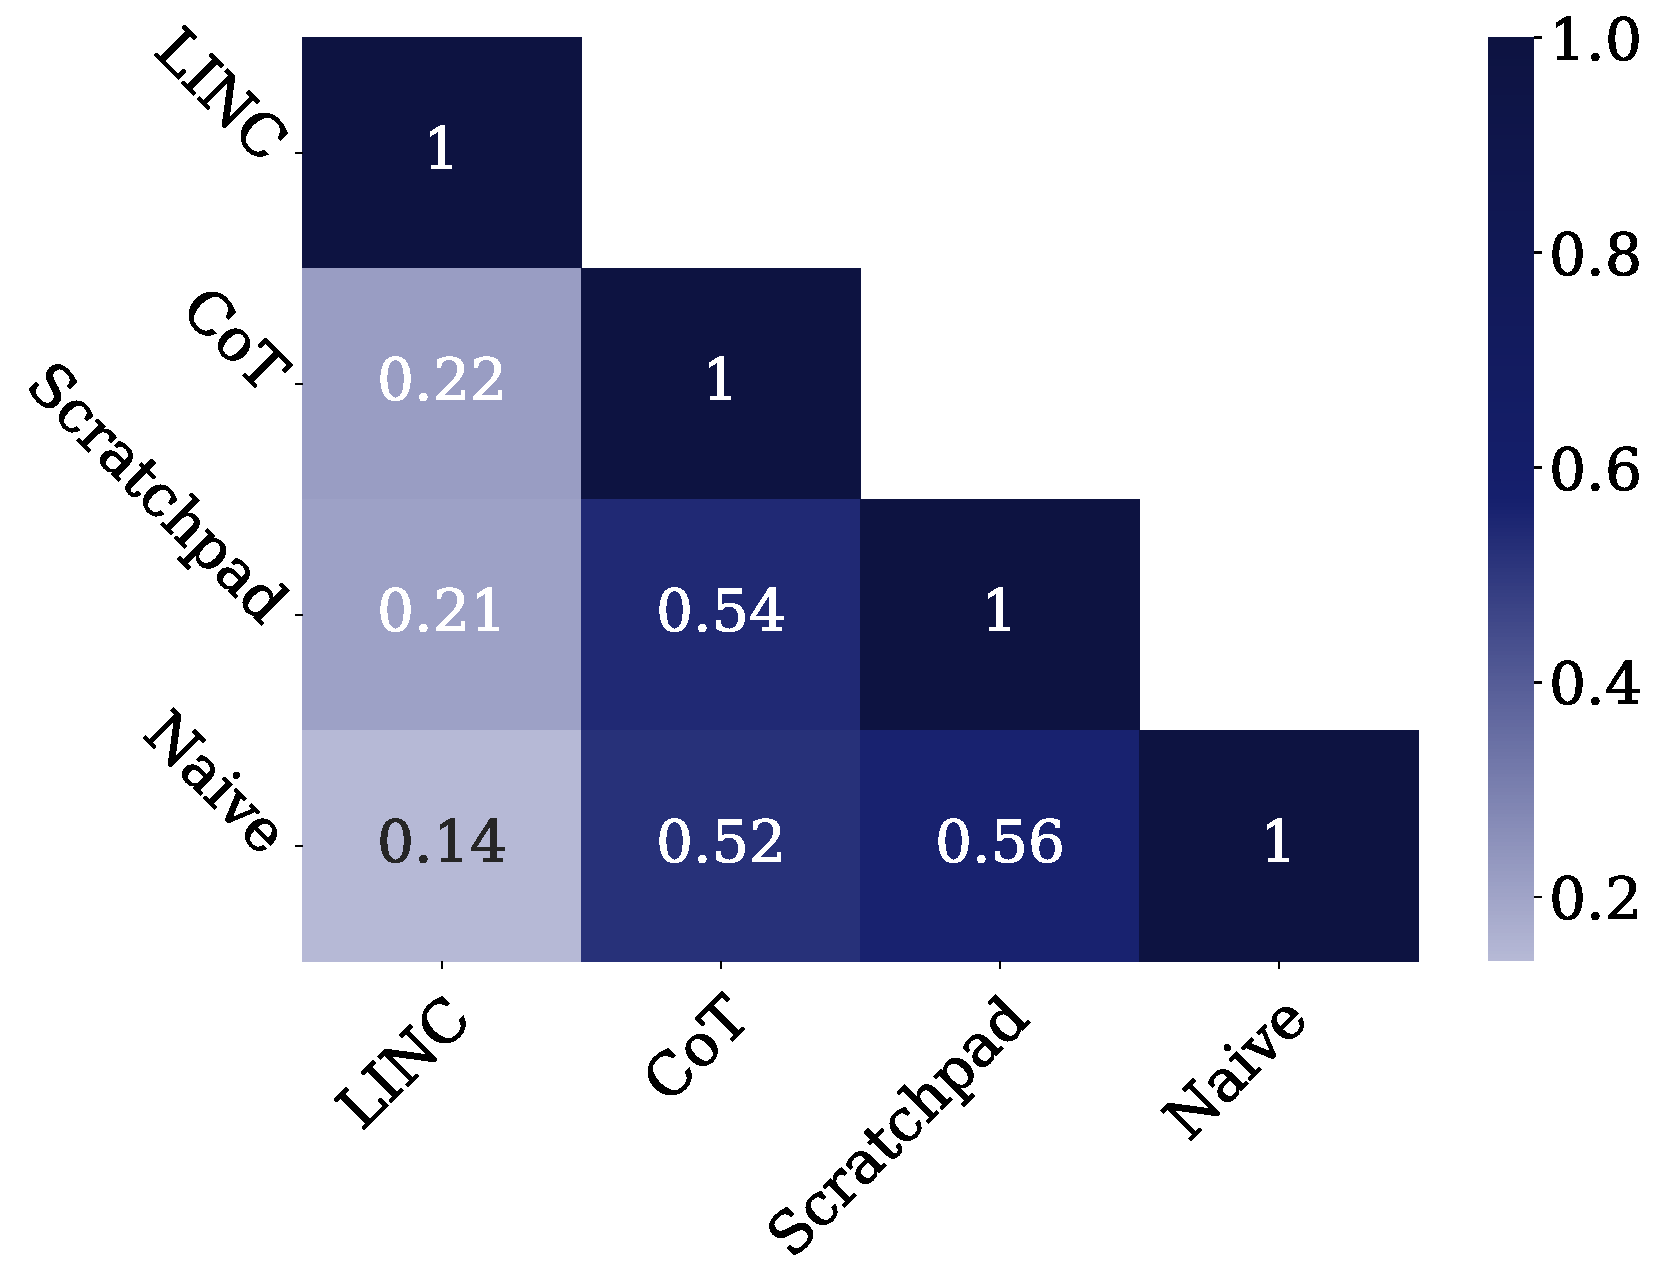
\includegraphics[width=\textwidth]{figures/matrices/gpt-4_method_similarity.pdf}
    \caption{Similarity between incorrect predictions of each method, i.e., \texttt{(A wrong == B wrong) / (A wrong or B wrong).}}
    \label{linc-paper:fig:method_similarity}
  \end{subfigure}

  \caption{Analyzing and comparing the mistakes made by GPT-4 on the FOLIO dataset.}
  \label{linc-paper:fig:confusion_plots}
\end{figure}

%%%
\subsection{Error Analysis}
\label{linc-paper:sec:error_analysis}
Having established that \texttt{LINC} can improve performance in many settings, we now move on to our final research question:
\textit{How do the failure modes of \texttt{LINC} compare to those of in-context reasoning methods}?
We focused on comparing GPT-4+\texttt{CoT} vs. GPT-4+\texttt{LINC} on FOLIO, since their overall performance was very similar (75.3\% vs. 72.5\% average accuracy). We leave an analysis of StarCoder+'s predictions on FOLIO to the original paper appendix.

\subsubsection{Qualitative Analysis} \label{linc-paper:sec:error_qualitative}
Qualitatively, we found that \texttt{LINC} and \texttt{CoT} had completely different failure modes. We give a high-level overview and abbreviated examples of each failure mode here, leaving full detailed examples to the original paper appendix.

First, we detail the failure modes for \texttt{LINC}:

\textbf{L1: FOL fails to capture implicit information not mentioned in the premises.} Often, there is obvious information not explicitly listed in the premises that is necessary to explicitly encode in FOL in order to successfully make a desired deduction. For example, in the snippet below one must encode in FOL the implicit assumption that Harry is a person (\texttt{Person(Harry)}).

\begin{itemize}
\itemsep0.1em
    \item[] \small Premise 1: \texttt{When a person reads a book, that person gains knowledge.}
    \item[] \small FOL: \parbox[t]{0.78\linewidth}{\ttfamily\small all x. all y. (Person(x) \& Reads(x, y) \& Book(y) ->\\ Gains(x, Knowledge))}
    \item[] \small Premise 2: \texttt{Harry read the book "Walden" by Henry Thoreau.}
    \item[] \small FOL: \texttt{Reads(Harry, Walden)}
    \item[] \small Conclusion (Prover9: Uncertain): \texttt{Harry gains knowledge.}
    \item[] \small FOL: \texttt{Gains(Harry, Knowledge)}
\end{itemize}


\textbf{L2: FOL fails to capture information explicitly mentioned in the premises due to the choice of representation.} Even when information is explicitly written in the premises, the choice of how the NL is represented in FOL can lead to lost information. In the example below, the fact that Heinrich was a Nazi German politician is captured by one symbol \texttt{NaziGermanPolitician}, causing the information that he was independently Nazi, German, or a politician to be lost.
As a result, \texttt{LINC} predicted \texttt{Uncertain} instead of the ground truth label \texttt{True}.

\begin{itemize}
\itemsep0.1em
    \item[] \small Premise: \texttt{Heinrich Schmidt was a Nazi German politician.}
    \item[] \small FOL: \texttt{NaziGermanPolitician (HeinrichSchmidt)}
    \item[] \small Conclusion (Prover9: Uncertain): \texttt{Heinrich Schmidt was German.}
    \item[] \small FOL: \texttt{German(HeinrichSchmidt)}
\end{itemize}

\textbf{L3: FOL contains syntax errors.}  Across all generations, we found that the FOL expressions sometimes contained syntax errors: 38\% for StarCoderPlus, 24\% for GPT-3.5, and 13\% for GPT-4. The most common error is that the same symbol is used with multiple arities. As an example, if \texttt{Summer(July4)} and \texttt{Loves(Alex, Summer)} were both present in a FOL translation, \texttt{Summer} would have a multiple arity violation.

Next, we detail three failure modes for \texttt{CoT}:

\textbf{C1: \texttt{CoT} concludes something different than it suggests.} One common mistake we often saw with the \texttt{CoT} approach was that it generated a chain of reasoning indicating uncertainty, but then asserted that the conclusion was false. An example of this is shown below, where GPT-4 suggested there was ``no evidence'' for the conclusion but then deduced it false.

\begin{lstlisting}[breaklines=true,basicstyle=\small\ttfamily]
Premises:
Some mammals have teeth.
Platypus have no teeth.
Platypus are mammals.
Humans have teeth.

Conclusion:
Platypus are reptiles.

(GPT-4 Incorrect CoT): Let's think step by step. We want to evaluate if platypus are reptiles. We know from the premises that platypus are mammals and that they have no teeth. The fact that some mammals have teeth does not contradict the fact that platypus, although mammals, do not have teeth. Moreover, the statement about humans having teeth is unrelated to the classification of platypus. There's no evidence in the premises that would suggest platypus are reptiles. Therefore, the statement is false.
\end{lstlisting}

\textbf{C2: CoT makes incorrect logical deductions.} While there were many instances where \texttt{CoT} made incorrect logical deductions, one common deduction mistake was the structure ``if $B$ is true and $A \rightarrow B$, then $A$ is true''. In the example shown below, we saw this incorrect deduction where A is ``Mike has an F1 visa'' and B is ``Mike needs to apply for CPT or OPT if he wants to work in the US''. We note that making this type of logical mistake is often called the \emph{fallacy of the converse}, and that humans are not immune to it, either.

\begin{lstlisting}[breaklines=true,basicstyle=\small\ttfamily]
Premises:
International students in US have either an F1 visa or a J1 visa.
An international student in US with an F1 visa needs to apply for CPT or OPT if the student wants to work in the US.
Mike is an international student.
Mike needs to apply for CPT if he wants to work in the US.

Conclusion (Ground Truth: Uncertain):
Mike has an F1 visa.

(GPT-4 Incorrect CoT): Let's think step by step. We want to evaluate if Mike has an F1 visa. From the premises, we know that Mike is an international student and needs to apply for CPT if he wants to work in the US. We also know that an international student in the US with an F1 visa needs to apply for CPT or OPT if the student wants to work in the US. So, it is clear that Mike has an F1 visa since he fits the criteria. Therefore, the conclusion is true.
\end{lstlisting}

\textbf{C3: \texttt{CoT} fails to find complex paths of reasoning.} We found that with all three models, \texttt{CoT} failed when the path of reasoning necessary to make the deduction was complex. Sometimes, \texttt{CoT} had difficulty getting started, and other times, it got stuck in the middle of a reasoning chain.

\subsubsection{Quantitative Analysis}

\textbf{1. Compared to \texttt{CoT}, \texttt{LINC} has worse recall but better precision on \texttt{True}/\texttt{False} predictions.} To see this,
we plotted the confusion matrices in Figure~\ref{linc-paper:fig:gpt_cot_confusion} (\texttt{CoT}) and Figure~\ref{linc-paper:fig:gpt_neurosym_confusion} (\texttt{LINC}).
Looking just at the distributions of predicted labels of the two methods, we saw that \texttt{CoT} predicted 32\% \texttt{True}, 27\% \texttt{False}, and 41\% \texttt{Uncertain}, while \texttt{LINC} predicted 24\% \texttt{True}, 17\% \texttt{False}, and 57\% \texttt{Uncertain} (with 2\% of predictions throwing an error).
Notably, we observed that \texttt{LINC} predicted \texttt{Uncertain} much more frequently than \texttt{CoT} (57\% vs. 41\%).
To understand why, note that the translation from natural language to FOL is a lossy process: recall that in L1 and L2, we saw that the information conveyed through the FOL is sometimes a subset of the information in the original premises. Removing pieces of crucial information that were on the critical path to deducing \texttt{True}/\texttt{False} may then leave an uncertain conclusion.
At the same time, while the FOL translations sometimes do not retain all of the information in the NL, they rarely contain false information that was not provided in the original premises.
Therefore, \texttt{LINC}'s precision when predicting \texttt{True} or \texttt{False} is very high (93\%) compared to that of \texttt{CoT} (81\%), but this comes at the cost of lower recall on \texttt{True}/\texttt{False} predictions (60\% for \texttt{LINC} vs. 75\% for \texttt{CoT}).

\textbf{2. \texttt{LINC} and \texttt{CoT} mispredict on different examples.} Earlier in Sec. \ref{linc-paper:sec:error_qualitative}, we saw that \texttt{LINC} and \texttt{CoT} exhibited different failure modes, which suggested they should fail on different examples. Indeed, we found that this was the case in our experiments on FOLIO:
Figure~\ref{linc-paper:fig:gpt_cot_neurosym} shows a $2\times2$ confusion matrix which compares whether or not each method's prediction was correct.
We observed that out of the $24+29+21=74$ samples where at least one method made an incorrect prediction, only 21 were shared.
On a closer examination of these 21 samples, we found that 16 were ambiguous or incorrect in their specification (details in the original paper appendix), so \textit{the two methods only agreed on 5 well-formed samples}.
This suggests that \texttt{LINC} and \texttt{CoT} are complementary methods which fail under distinct circumstances.

\textbf{3. Mispredictions of in-context reasoning baselines are more similar to each other than they are with mispredictions of \texttt{LINC}.} As an extension of the previous analysis, we next investigated the correlation between the mispredictions of each pair of methods.
To do so, we define a similarity score between two methods $A$ and $B$ as follows:
Given a dataset $D$ with $N$ rows and ground truth labels $\{A_i\}_{i=1}^N$ and $\{B_i\}_{i=1}^N$ from two methods $A$ and $B$, we define
$$\text{sim}_D(A, B) \triangleq \frac{\sum_{i=1}^N \mathbf{1}\left[ A_i = B_i \ne R_i \right] }{\sum_{i=1}^N \mathbf{1}\left[ A_i \ne R_i \text{ or } B_i \ne R_i\right]}$$
In words, $\text{sim}_D(A,B)$ measures the number of instances where $A$ and $B$ are wrong in identical ways vs. the number of instances where \emph{at least one} of them is wrong.

Figure~\ref{linc-paper:fig:method_similarity} shows the pairwise similarity between our four methods, highlighting that the similarity between \texttt{LINC}'s mispredictions and the other methods' mispredictions ($0.14$, $0.21$, $0.22$) is much lower than the similarity between any pair of the in-context reasoning methods ($0.52$, $0.54$, $0.56$).
These results suggest that for GPT-4 on FOLIO, \texttt{LINC} was the only method we evaluated which significantly altered the ways in which the model \emph{fails} to reason.
